\documentclass[12pt]{article}
\usepackage[letterpaper, top=1.25in, bottom=1.25in, left=1in, right=1in]{geometry}
\usepackage{fancyhdr} % http://ctan.org/pkg/fancyhdr
\usepackage{hyperref}
% \usepackage{xcolor}
\usepackage{graphicx}
\usepackage{indentfirst}
\usepackage[export]{adjustbox}

% % % % % % % % % % % % 
% Citation formatting %
% % % % % % % % % % % % 

\usepackage[style=ieee]{biblatex}
\addbibresource{sources.bib}

% % % % % % % % %
% Hyperlinking  %
% % % % % % % % %

\hypersetup{
    colorlinks=false, % set true if you want colored links
    linktoc=all,     % set to all if you want both sections and subsections linked
    % linkcolor=black,  %c hoose some color if you want links to stand out
    % citecolor=black
    % urlcolor=black
}

% % % % % % % % % % % % % % % %
% Global title, author, date  %
% % % % % % % % % % % % % % % %

\title{Exploring Smart Sensor Systems}
\author{Nathan Quadras \& Kosta Sergakis}
% \author1{Quadras \& Sergakis}
% \date{\today}
\date{April 30, 2025}
\makeatletter
\let\runauthor\@author
\let\runtitle\@title
\let\rundate\@date
\makeatother

% % % % % % % % % % %
% Header and Footer %
% % % % % % % % % % %

\pagestyle{fancy} % change page style to fancy
\fancyhf{} % clear header/footer
\setlength{\headheight}{15pt}
\fancyhead[L]{Quadras \& Sergakis}
\fancyhead[C]{\runtitle}
\fancyhead[R]{\rundate}
\fancyfoot[C]{\thepage} % \fancyfoot[R]{\thepage}
\renewcommand{\headrulewidth}{0.4pt} % default \headrulewidth is 0.4pt
\renewcommand{\footrulewidth}{0.4pt} % default \footrulewidth is 0pt

% \usepackage{natbib}
\begin{document}

    % % % % % % % %
    % Title Page  %
    % % % % % % % %
    
    \begin{titlepage}
        \begin{center}
            \vspace*{1.5cm}
            
            \textbf{\runtitle}
            
            \vspace{1cm}
            
            An exploration of:\\
            \vspace{0.25cm}
            Slip Angle Sensors
                
            \vspace{1cm}
            
            \textbf{\runauthor}
            
            \vfill  
            
            \vspace{1cm}

            
\includegraphics[width=0.4\textwidth]{resources/michigan-state-logo-png-transparent.png}
                
            Electrical and Computer Engineering\\
            Michigan State University\\
            East Lansing, Michigan\\
            \rundate
                
        \end{center}
    
    \end{titlepage}


    % % % % % % % % % % %
    % Table of Contents %
    % % % % % % % % % % %

    \setcounter{secnumdepth}{0} % removes section numbers
    % \maketitle
    
    \tableofcontents
    
    \newpage

    \section{Introduction}
        
    Vehicles are more attainable than ever and are advancing quickly. Modern cars 
    are equipped with sophisticated systems that enhance performance, safety, and driver 
    comfort. Vehicle dynamics is a tremendous topic and an area of growing interest, especially 
    as more automated driving technologies emerge. Vehicle dynamics is the study of vehicle 
    motion in relevant user operations \autocite{Jacobson_2016}, which encompasses factors like kinematics, forces, 
    and moments acting on a vehicle during acceleration, braking and steering. The core of vehicle 
    dynamics involves the following primary aspects: the mechanisms that disturb a vehicle’s state 
    (inputs) and the mechanisms through which the vehicle responds (outputs). Arguably the most 
    critical aspect of vehicle dynamics is tire behavior, specifically how a tire generates lateral 
    force during cornering. Central to this behavior is the concept of slip angle – the difference 
    between the direction a vehicle is traveling and the direction that the body of the vehicle is 
    pointing (heading vs. true heading) \autocite{Racelogic_2015}. Understanding slip angle is essential for analyzing 
    handling characteristics, improving stability control systems, and optimizing driver feedback.
        
        \subsection{Vehicle Dynamics}

        Performance driving, autonomous driving and regular commuter driving all require the same characteristic: 
        control. Controllable vehicles are what makes rapid maneuvers possible. On the other hand, the required 
        motion must be stable to maintain directional stability under disturbances \autocite{MMM}. 

        \begin{center}
            \vspace{0.5cm}

            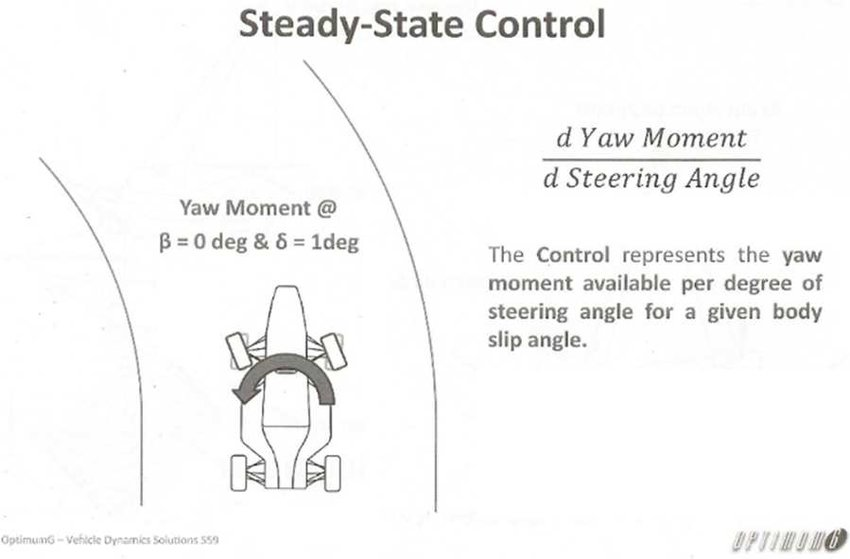
\includegraphics[width=0.7\textwidth]{resources/Defining-of-control-Claude-Rouelle-Applied-VD-seminar.png}

            \vspace{0.5cm}

            \textbf{Figure 1: Definition of Control} \autocite{MMM}
            \label{control}
        
        \end{center}

        \begin{center}
            \vspace{0.5cm}

            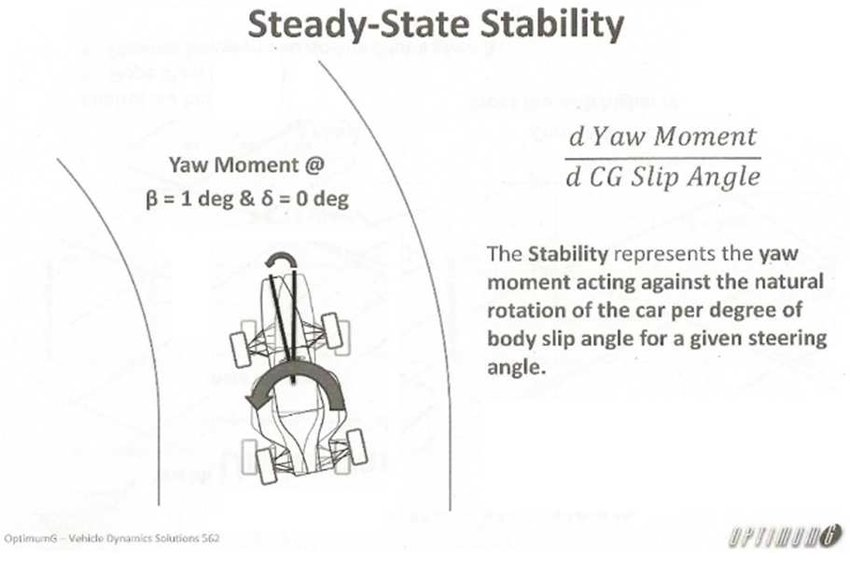
\includegraphics[width=0.7\textwidth]{resources/Defining-of-stability-Claude-Rouelle-Applied-VD-seminar.png}

            \vspace{0.5cm}

            \textbf{Figure 2: Definition of Stability} \autocite{MMM}
            \label{stability}
        
        \end{center}

        It is crucial to define the tractive limit of the vehicle, or the “safety margin” to determine the range of 
        possible motions that the vehicle can produce while maintaining stability \autocite{MMM}. Slip angle is incredibly important 
        because it enables the concepts mentioned above. In other words, slip angle determines vehicle maneuverability. If 
        slip angle is observed, various states of the vehicle can be determined. 

        \begin{center}
            \vspace{0.5cm}

            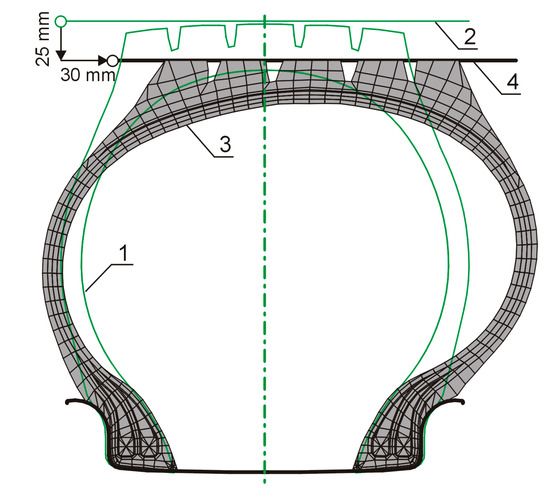
\includegraphics[width=0.5\textwidth]{resources/applsci-10-04326-g009-550.jpg}

            \vspace{0.5cm}

            \textbf{Figure 3: Tire Deformation} \autocite{app10124326}
            \label{tire_deformation_1}
        
        \end{center}

        \begin{center}
            \vspace{0.5cm}

            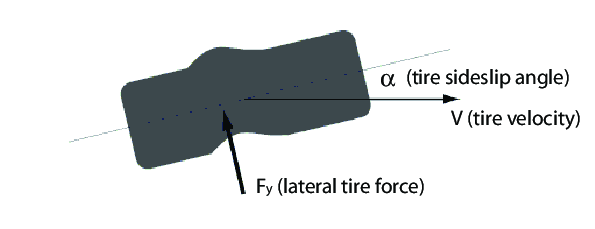
\includegraphics[width=0.8\textwidth]{resources/Lateral-tire-deformation.png}

            \vspace{0.5cm}

            \textbf{Figure 4: Tire Deformation} \autocite{inproceedings}
            \label{tire_deformation_2}
        
        \end{center}

        \begin{center}
            \vspace{0.5cm}

            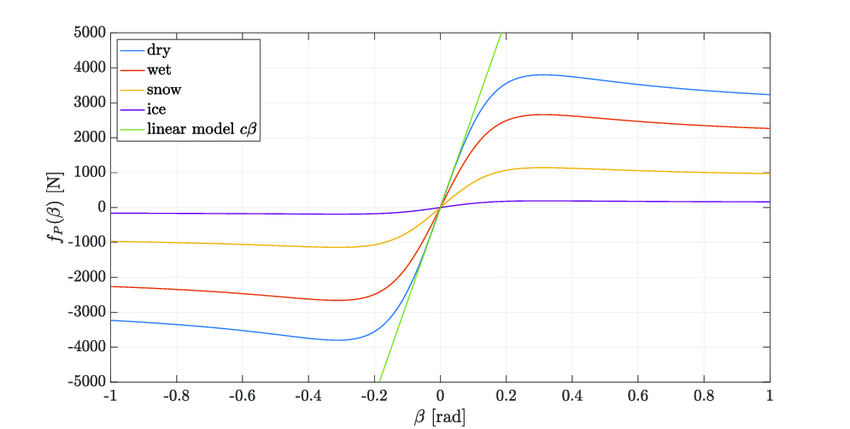
\includegraphics[width=1\textwidth]{resources/Pacejkas-tire-model.png}

            \vspace{0.5cm}

            \textbf{Figure 5: Example Pacejka Tire Model} \autocite{pacejka}
            \label{pjka}
        
        \end{center}

        \begin{center}
            \vspace{0.5cm}

            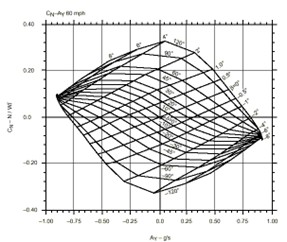
\includegraphics[width=0.5\textwidth]{resources/tn_MMM807.jpg}

            \vspace{0.5cm}

            \textbf{Figure 6: MMM} \autocite{Milliken_Research_Associates}
            \label{MMMa}
        
        \end{center}

        A common way to observe/determine the limits of a vehicle is through a Yaw Moment Diagram, or the MRA Moment Method 
        (MMM) \hyperref[MMMa]{[Figure 6]} \autocite{Milliken_Research_Associates}. A critical component of the Yaw Moment Diagram would be the quantification of the forces necessary to hold 
        a vehicle through a turn. As shown in  \hyperref[tire_deformation_2]{figure 4}, a primitive to determining the lateral force of a tire is the slip angle. 
        Pacejka’s formula can display the relationship between slip angle and lateral tire force as shown in \hyperref[pjka]{figure 5}. Ultimately, 
        the goal is to determine the limits of the vehicle to prevent drivers from reaching the point of no return; a loss of 
        stability, leading to control being removed from the driver.

        \subsection{Overview \& Motivation}
        
        This smart system focuses on real-time slip angle estimation and control for ground vehicles. Accurate knowledge of 
        slip angle enables Advanced Drive-Assistance Systems (ADAS), traction control, and autonomous driving algorithms to make 
        more informed decisions when navigating corners, avoiding obstacles, or maintaining control on low-friction surfaces. 
        
        The motivation for this system stems from the growing demand for safer and more responsive vehicles in both human-driven 
        and autonomous applications. While modern vehicles are equipped with various sensors, slip angle is notoriously expensive 
        to measure directly due to the niche, specialized equipment involved. By designing a smart system capable of observing slip 
        angle in real-time using accessible components, this solution offers a cost-effective and scalable method to improve vehicle 
        safety, performance, and driver confidence across a wide range of driving conditions. 

    \section{System Level Design}
        \subsection{Microcontroller (Teensy 4.0)}
        \subsection{Optical Sensor (PAW3515DB)}
        \subsection{Inertial Measurement Unit (BNO055)}
        \subsection{RGB LED}
    \section{Software Design}
    % % % % % % % % %
    % Bibliography  %
    % % % % % % % % %

    % \addcontentsline{toc}{section}{Works Cited}
    % \printbibliography
    \newpage
    \phantomsection % Create a phantom section to get the correct page number in the ToC
    \addcontentsline{toc}{section}{Works Cited}
    \printbibliography[title=Works Cited]

    % \bibliographystyle{plainnat}
    % \bibliography{sources}

\end{document}